\documentclass[border=4pt]{standalone}
\usepackage{amsmath,amssymb,amsfonts}
\usepackage{xcolor,colortbl,array,booktabs,multirow}
\usepackage{tikz}
\usepackage{pgfplots}
\pgfplotsset{compat=1.16}
\usetikzlibrary{arrows, automata, backgrounds, calendar, chains, decorations,
    matrix, mindmap, patterns, petri, positioning, shadows, shapes.geometric,
    trees, shapes, decorations.pathreplacing, calc, tikzmark, arrows.meta,
    intersections, fit, graphs, quotes, angles, decorations.markings}
\newcommand{\st}{\text{ s.t. }}
\newcommand{\x}{\mathbf{x}}
\renewcommand{\b}{\mathbf{b}}
\renewcommand{\c}{\mathbf{c}}
\newcommand{\A}{\mathbf{A}}
\newcommand{\y}{\mathbf{y}}
\newcommand{\z}{\mathbf{z}}
\newcommand{\R}{\mathbb{R}}
\newcommand{\RR}{\mathbb{R}}
\newcommand{\Z}{\mathbb{Z}}
\newcommand{\ZZ}{\mathbb{Z}}
\newcommand{\npcomplete}{NP-complete}
\providecommand{\true}{\text{TRUE}}
\providecommand{\false}{\text{FALSE}}
\tikzset{vertex/.style={circle,fill=black!25,minimum size=20pt,inner sep=0pt},
    edge/.style={draw,thick,-},weight/.style={font=\small},
    selected vertex/.style={vertex, fill=red!24},
    selected edge/.style={draw,line width=2pt,-,red!50},
    ignored edge/.style={draw,line width=2pt,-,black!20}}
\newcommand{\vect}{\vec}
\providecommand{\ds}{\displaystyle}
\providecommand{\longvect}{\overrightarrow}
\usepackage[normalem]{ulem}
\definecolor{ocre}{RGB}{243,102,25}
\providecommand{\leftB}{\left[}
\providecommand{\rightB}{\right]}
\tikzset{directed/.style={postaction={decorate,decoration={markings,mark=at position .65 with {\arrow{>}}}}},
    directed1/.style={postaction={decorate,decoration={markings,mark=at position .65 with {\arrow{>}}}}}}
\begin{document}
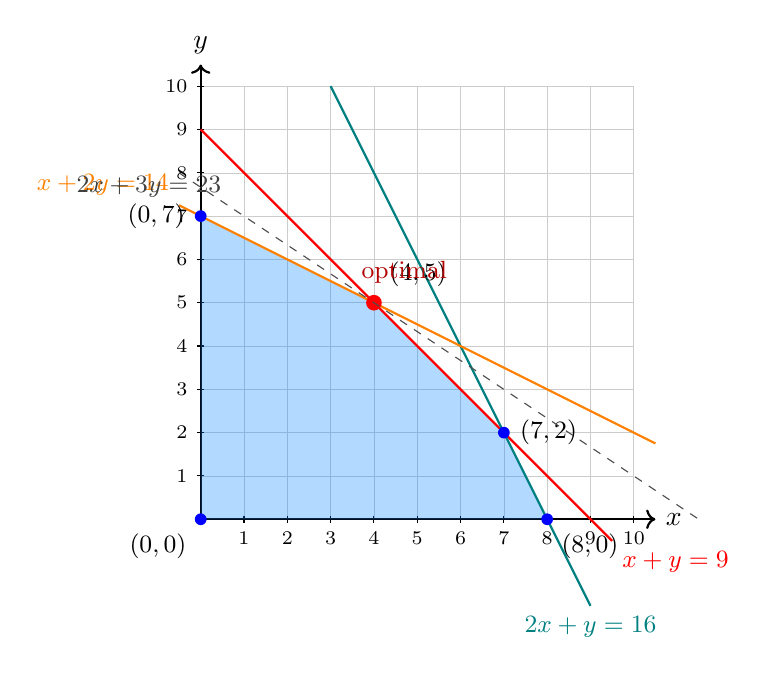
\begin{tikzpicture}[scale=0.55]
    % Grid and axes
    \draw[gray!40, very thin, step=1] (0,0) grid (10,10);
    \draw[->, thick] (0,0) -- (10.5,0) node[right] {$x$};
    \draw[->, thick] (0,0) -- (0,10.5) node[above] {$y$};
    \foreach \x in {1,...,10} \draw (\x,0.08) -- (\x,-0.08) node[below] {\scriptsize \x};
    \foreach \y in {1,...,10} \draw (0.08,\y) -- (-0.08,\y) node[left] {\scriptsize \y};

    % Feasible region: (0,0) -- (8,0) -- (7,2) -- (4,5) -- (0,7) -- cycle
    \fill[blue!50!cyan, opacity=0.3]
        (0,0) -- (8,0) -- (7,2) -- (4,5) -- (0,7) -- cycle;

    % Constraint boundary lines, extended a bit beyond the polygon
    % x + y = 9 (red): from (0,9) to (9,0)
    \draw[red, thick] (0,9) -- (9.5,-0.5) node[below right] {\small $x+y=9$};
    % 2x + y = 16 (teal): from (0,16) clipped, take (3,10) to (9,-2)
    \draw[teal, thick] (3,10) -- (9,-2) node[below] {\small $2x+y=16$};
    % x + 2y = 14 (orange): from (0,7) to (14,0)
    \draw[orange, thick] (-0.5,7.25) node[above left] {\small $x+2y=14$} -- (10.5,1.75);

    % Vertices
    \node[fill=blue,circle,inner sep=1.5pt,label={below left:\small$(0,0)$}]   at (0,0) {};
    \node[fill=blue,circle,inner sep=1.5pt,label={below right:\small$(8,0)$}]  at (8,0) {};
    \node[fill=blue,circle,inner sep=1.5pt,label={right:\small$(7,2)$}]        at (7,2) {};
    \node[fill=red, circle,inner sep=2pt,  label={above right:\small$(4,5)$}]  at (4,5) {};
    \node[fill=blue,circle,inner sep=1.5pt,label={left:\small$(0,7)$}]         at (0,7) {};

    % Optimal point and objective level set 2x + 3y = 23 (dashed)
    % line passes through (4,5): 8 + 15 = 23. Endpoints: (11.5,0) and (-0.5, 8)
    \draw[dashed, gray!60!black]
        (-0.5,8) -- (11.5,0) node[pos=0.1, above left, gray!50!black]
        {\small $2x+3y=23$};
    \node[draw=none, red!70!black] at (4.7,5.7) {\small optimal};
\end{tikzpicture}
\end{document}
